\documentclass{csse4400}

% \teachermodetrue

\usepackage{float}

\usepackage{languages}

\title{Load Testing \& Bottlenecks}
\author{Brae Webb}

\date{\week[practical]{8}}
\begin{document}

\maketitle

\begin{figure}[h]
    \centering
    
\includegraphics[width=0.8\textwidth]{images/bottleneck}
\end{figure}

\section{This Week}
Our goal is to:
\begin{itemize}
  \item Introduce structured logging to TaskOverflow.
  \item Deploy TaskOverflow to AWS.
  \item Write k6 tests to ensure TaskOverflow can handle given scenarios.
  \item Uncover and fix bottlenecks in the TaskOverflow application using the logs.
\end{itemize}

\section{Watchtower}
In this course we have repeatedly claimed that there is value in montoring and logging.
This week, we aim to prove it by using logging to help diagnose issues with a deployment of TaskOverflow.
For this task, we have integrated \link{Watchtower}{https://pypi.org/project/watchtower/} into the project.
Watchtower is a Python library that allows us to send logs to AWS CloudWatch,
allowing us to monitor the applications performance in real time.

Currently the project is configured to log API accesses made with Flask and to log database queries created by SQL Alchemy.
This results in an unstructured log stream as seen in Figure \ref{fig:cloud-logs}.

\begin{figure}[ht]
    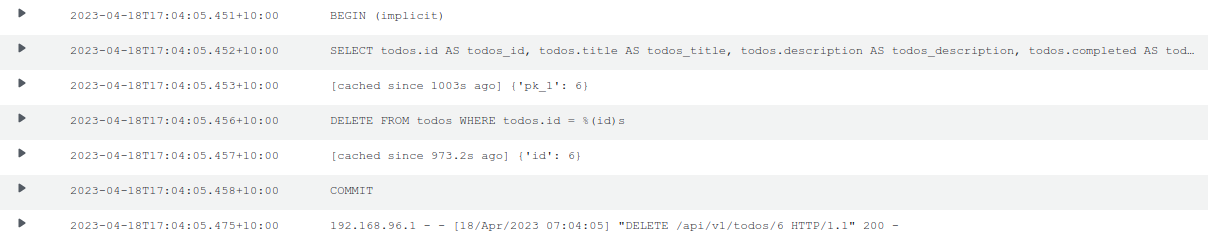
\includegraphics[width=\textwidth]{images/cloud-watch-log}
    \caption{An example of logs made to AWS CloudWatch for a DELETE request in the TaskOverflow API.}
    \label{fig:cloud-logs}
\end{figure}

\paragraph{Getting Started}
\begin{enumerate}
    \item Using the GitHub Classroom link for this practical provided by your tutor in Slack, create a repository to work within.
    \item Install Terraform if not already installed, as it will be required again this week.
    \item Start your learner lab and copy the AWS Learner Lab credentials into a credentials file in the root of the repository.
\end{enumerate}

\paragraph{What's New}
We are returning to TaskOverflow roughly from the state at the end of the last practical.
The following notable changes have been made:
\begin{itemize}
    \item \texttt{Watchtower} has been installed as a dependency.
    \item In \texttt{docker-compose.yml}, we mount the \texttt{credentials} file to \texttt{/root/.aws/credentials}.
        This allows local testing of \texttt{watchtower} to log to AWS CloudWatch.
    \item Logging has been introduced for Flask and SQL Alchemy.
\end{itemize}

Our first task will be to replicate the above logs in Figure \ref{fig:cloud-logs}.
Once you have copied \texttt{credentials} into the project root,
start docker compose with:
\bash{docker-compose up}

\begin{code}[numbers=none]{}
app_1       |  * Serving Flask app 'todo'
app_1       |  * Debug mode: on
app_1       | INFO:werkzeug:WARNING: This is a development server. Do not use it in a production deployment. Use a production WSGI server instead.
app_1       |  * Running on all addresses (0.0.0.0)
app_1       |  * Running on http://127.0.0.1:6400
app_1       |  * Running on http://192.168.96.3:6400
app_1       | INFO:werkzeug:Press CTRL+C to quit
app_1       | INFO:werkzeug: * Restarting with stat
app_1       | INFO:botocore.credentials:Found credentials in shared credentials file: ~/.aws/credentials
app_1       | INFO:sqlalchemy.engine.Engine:select pg_catalog.version()
app_1       | INFO:sqlalchemy.engine.Engine:[raw sql] {}
app_1       | INFO:sqlalchemy.engine.Engine:select current_schema()
app_1       | INFO:sqlalchemy.engine.Engine:[raw sql] {}
app_1       | INFO:sqlalchemy.engine.Engine:show standard_conforming_strings
app_1       | INFO:sqlalchemy.engine.Engine:[raw sql] {}
app_1       | INFO:sqlalchemy.engine.Engine:BEGIN (implicit)
app_1       | INFO:sqlalchemy.engine.Engine:SELECT pg_catalog.pg_class.relname
app_1       | FROM pg_catalog.pg_class JOIN pg_catalog.pg_namespace ON pg_catalog.pg_namespace.oid = pg_catalog.pg_class.relnamespace
app_1       | WHERE pg_catalog.pg_class.relname = %(table_name)s AND pg_catalog.pg_class.relkind = ANY (ARRAY[%(param_1)s, %(param_2)s, %(param_3)s, %(param_4)s, %(param_5)s]) AND pg_catalog.pg_table_is_visible(pg_catalog.pg_class.oid) AND pg_catalog.pg_namespace.nspname != %(nspname_1)s
app_1       | INFO:sqlalchemy.engine.Engine:[generated in 0.00011s] {'table_name': 'todos', 'param_1': 'r', 'param_2': 'p', 'param_3': 'f', 'param_4': 'v', 'param_5': 'm', 'nspname_1': 'pg_catalog'}
app_1       | INFO:sqlalchemy.engine.Engine:COMMIT
app_1       | WARNING:werkzeug: * Debugger is active!
\end{code}

You should see logs similar to the above.
Notice that information about Flask is prefixed with \texttt{INFO:werkzeug} and information about SQL Alchemy is prefixed with \texttt{INFO:sqlalchemy.engine.Engine}.
This prefix indicates which log stream they are put into.

Open the AWS CloudWatch console and go to \texttt{Log groups} on the side panel.
You should see a log group called \texttt{taskoverflow},
if you click on that group you can see the two log streams.

\begin{center}
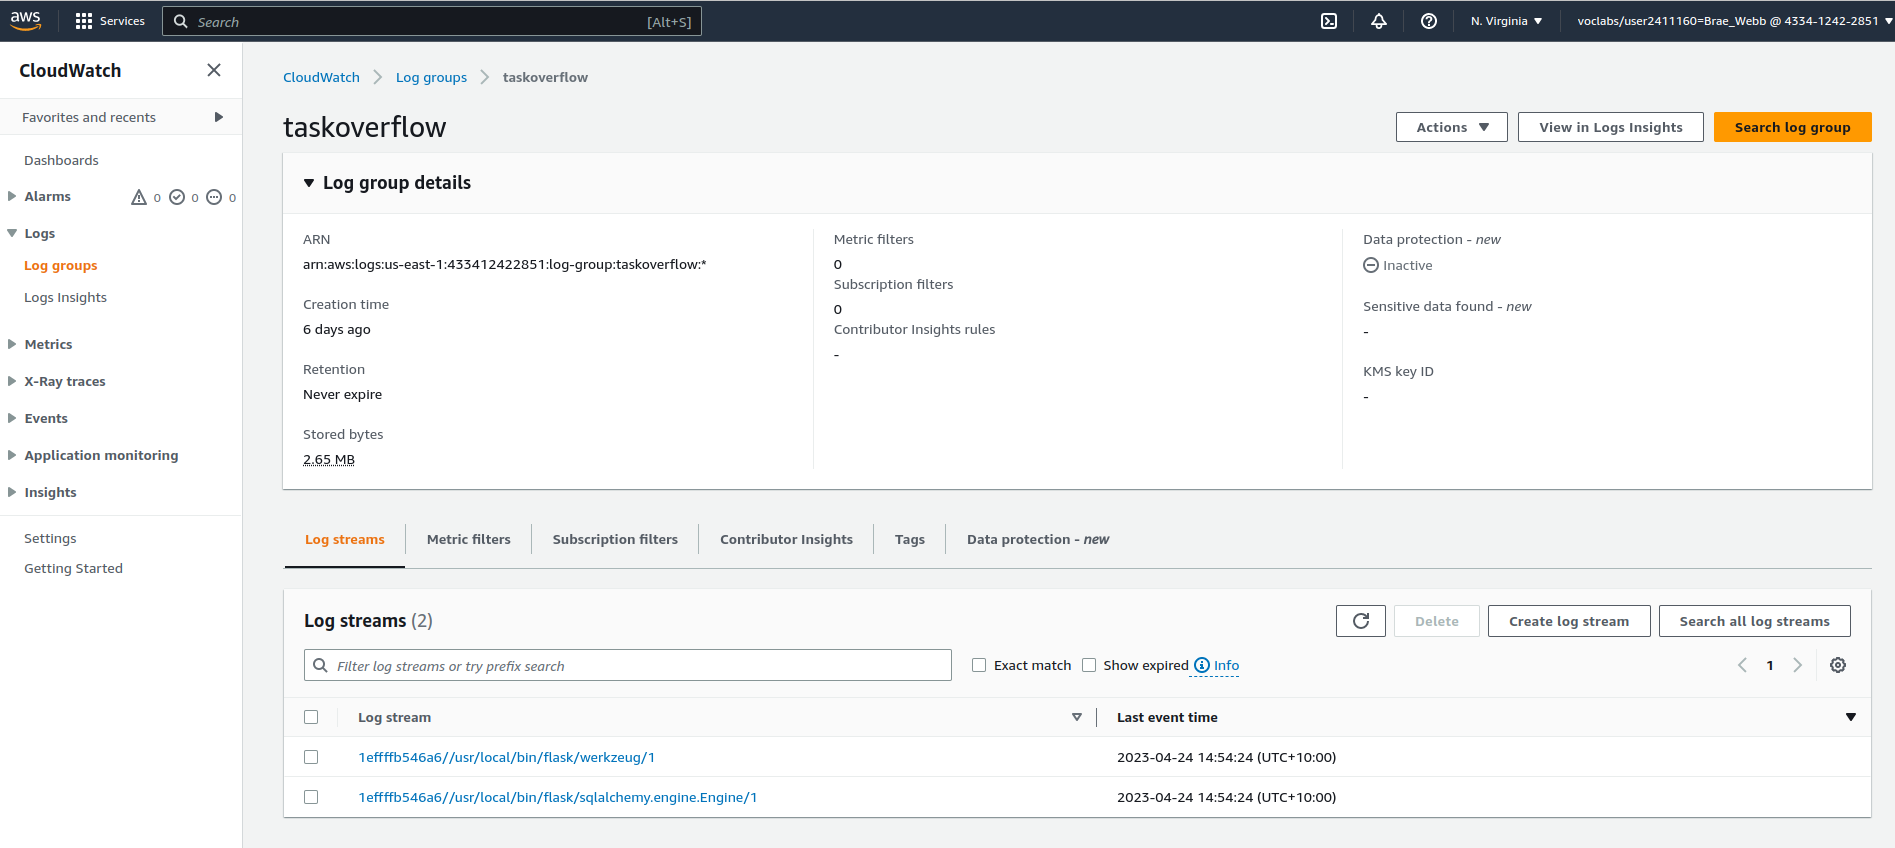
\includegraphics[width=0.8\textwidth]{images/log-group}
\end{center}

\subsection{Structured Logging}

Our first task will be to convert the current logging into a structured logging format.
As we saw in last weeks tutorial, structured logging can be as simple as logging a JSON object.
This allows logging services to quickly filter through logs based on criteria on the objects fields.

\subsection{Correlation IDs}

Correlation IDs are a mechanism to help understand the path of a request, event, message, etc. through a system.
When logging it can be helpful to be able to trace the execution of a particular request.

%\bibliographystyle{ieeetr}
%\bibliography{books,ours}

\end{document}
